\documentclass[user_manual.tex]{subfiles}

\begin{document}
 %Capitulo del Hardware
\chapter{Hardware} \label{aped.A}
En la siguiente sección mostramos el hardware utilizado para el desarrollo del robot Justina así como especificaciones
del mismo y algunas configuraciones que deben seguirse para su correcto funcionamiento.


\section{Actuadores y sus controladores}
En ésta sección se mostrar los componentes utilizados para ensamblar al robot Justina y especificaciones técnicas como
algunas configuraciones y recomendaciones del mismo para su correcto funcionamiento.


\subsection{Servomotor MX-106}

%Figura
\begin{center}
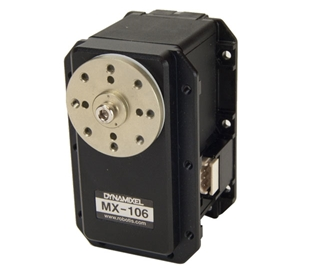
\includegraphics[width=0.35\textwidth]{Figures/Hardware/Partes/MX-106.png}
\captionof{figure}{MX-106}
\label{fig:Hardware:Partes:MX-106}
\end{center}

%Principio de la tabla del MX-106
\begin{table}[H]
\begin{center}
\begin{tabular}{|l|l|l|l|}%Define el número de columnas

\hline
\multicolumn{4}{|c|}{MX-106} \\ \hline %Une un renglon completo 
Voltaje de operación & 14.8[V] & 12[V] & 11.1[V]\\
\hline
\multirow{3}{1cm}{Torque} & 102[kg*cm] & 85.6[Kg*cm] & 81.5[kg*cm]\\ \cline {2-4} %Se hace un renglon multiple
& 10.0[N*m] & 8.4[N*m] & 8[N*m] \\ \cline{1-4}
Velocidad sin carga & 55[RPM] & 45[RPM] & 41[RPM]\\ 
\hline
Masa & \multicolumn{3}{|c|}{153[g]} \\ 
\hline
Medidas & \multicolumn{3}{|c|}{40.2[mm]x65.1[mm]x46[mm]} \\ 
\hline
Resolución & \multicolumn{3}{|c|}{0.088[grados]} \\ 
\hline
Radio de redicción & \multicolumn{3}{|c|}{1/225} \\ 
\hline
Ángulo de operación & \multicolumn{3}{|c|}{360 grados o giro continuo} \\ 
\hline
Corriente máxima & \multicolumn{3}{|c|}{5.2[A] @ 12[V]} \\ 
\hline
Corriente en espera & \multicolumn{3}{|c|}{55[mA]} \\ 
\hline
Temperatura de operación & \multicolumn{3}{|c|}{-5[C]~85[C]} \\ 
\hline
Protocolo & \multicolumn{3}{|c|}{TTL Asynchronous serial} \\ 
\hline
Límite de modulos & \multicolumn{3}{|c|}{254 direcciones validas} \\ 
\hline
Velocidad & \multicolumn{3}{|c|}{8000bps~3Mbps} \\
\hline
Realimentación de posición & \multicolumn{3}{|c|}{Sí} \\
\hline
Realimentación de temperatura & \multicolumn{3}{|c|}{Sí} \\
\hline
Realimentación de voltaje de carga & \multicolumn{3}{|c|}{Sí} \\
\hline
Realimentación de voltaje de entrada & \multicolumn{3}{|c|}{Sí} \\
\hline
PID & \multicolumn{3}{|c|}{Sí} \\
\hline
Materiales & \multicolumn{3}{|c|}{Engranes de metal y cuerpo plastico} \\
\hline
\multirow{4}{1cm}{Lista de controladores} & \multicolumn{3}{|c|}{USB2Dynamixel} \\ \cline {2-4} & \multicolumn{3}{|c|}{CM-530}\\ \cline {2-4} & \multicolumn{3}{|c|}{CM-700}\\ \cline {2-4} & \multicolumn{3}{|c|}{Arbotix}\\ \cline {1-4}
\hline

\end{tabular}
\caption{MX-106}
\label{Datos del MX-106}
\end{center}
\end{table}
%Fin de la tabla
 
 \subsection{Servomotor MX-64}

 %Figura
\begin{center}
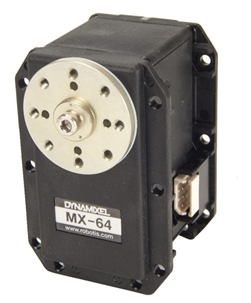
\includegraphics[width=0.25\textwidth]{Figures/Hardware/Partes/MX-64.png}
\captionof{figure}{MX-64}
\label{fig:Hardware:Partes:MX-64}
\end{center}

%Principio de la tabla del MX-64
\begin{table}[H]
\begin{center}
\begin{tabular}{|l|l|l|l|}%Define el número de columnas

\hline
\multicolumn{4}{|c|}{MX-64} \\ \hline %Une un renglon completo 
Voltaje de operación & 14.8[V] & 12[V] & 11.1[V]\\
\hline
\multirow{3}{1cm}{Torque} & 74[kg*cm] & 61[Kg*cm] & 56[kg*cm]\\ \cline {2-4} %Se hace un renglon multiple
& 7.3[N*m] & 6[N*m] & 5.5[N*m] \\ \cline{1-4}
Velocidad sin carga & 78[RPM] & 63[RPM] & 58[RPM]\\ 
\hline
Masa & \multicolumn{3}{|c|}{126[g]} \\ 
\hline
Medidas & \multicolumn{3}{|c|}{40.2[mm]x61.1[mm]x41[mm]} \\ 
\hline
Resolución & \multicolumn{3}{|c|}{0.088[grados]} \\ 
\hline
Radio de redicción & \multicolumn{3}{|c|}{1/200} \\ 
\hline
Ángulo de operación & \multicolumn{3}{|c|}{360 grados o giro continuo} \\ 
\hline
Corriente máxima & \multicolumn{3}{|c|}{4.1[A] @ 12[V]} \\ 
\hline
Corriente en espera & \multicolumn{3}{|c|}{100[mA]} \\ 
\hline
Temperatura de operación & \multicolumn{3}{|c|}{-5[C]~85[C]} \\ 
\hline
Protocolo & \multicolumn{3}{|c|}{TTL Asynchronous serial} \\ 
\hline
Límite de modulos & \multicolumn{3}{|c|}{254 direcciones validas} \\ 
\hline
Velocidad de transmisión & \multicolumn{3}{|c|}{8000bps~3Mbps} \\
\hline
Realimentación de posición & \multicolumn{3}{|c|}{Sí} \\
\hline
Realimentación de temperatura & \multicolumn{3}{|c|}{Sí} \\
\hline
Realimentación de voltaje de carga & \multicolumn{3}{|c|}{Sí} \\
\hline
Realimentación de voltaje de entrada & \multicolumn{3}{|c|}{Sí} \\
\hline
PID & \multicolumn{3}{|c|}{Sí} \\
\hline
Materiales & \multicolumn{3}{|c|}{Engranes de metal y cuerpo plastico} \\
\hline
\multirow{4}{1cm}{Lista de controladores} & \multicolumn{3}{|c|}{USB2Dynamixel} \\ \cline {2-4} & \multicolumn{3}{|c|}{CM-530}\\ \cline {2-4} & \multicolumn{3}{|c|}{CM-700}\\ \cline {2-4} & \multicolumn{3}{|c|}{Arbotix}\\ \cline {1-4}
\hline

\end{tabular}
\caption{MX-64}
\label{Datos del MX-64}
\end{center}
\end{table}
%Fin de la tabla

\subsection{Servomotor MX-28}

%Figura
\begin{center}
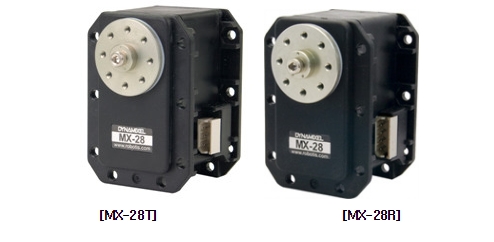
\includegraphics[width=0.6\textwidth]{Figures/Hardware/Partes/MX-28.png}
\captionof{figure}{MX-28}
\label{fig:Hardware:Partes:MX-28}
\end{center}

%Principio de la tabla
\begin{table}[H]
\begin{center}
\begin{tabular}{|l|l|l|l|}%Define el número de columnas

\hline
\multicolumn{4}{|c|}{MX-28} \\ \hline %Une un renglon completo 
Voltaje de operación & 14.8[V] & 12[V] & 11.1[V]\\
\hline
\multirow{3}{1cm}{Torque} & 31[kg*cm] & 25.5[Kg*cm] & 23.4[kg*cm]\\ \cline {2-4} %Se hace un renglon multiple
& 3.1[N*m] & 2.5[N*m] & 2.3[N*m] \\ \cline{1-4}
Velocidad sin carga & 67[RPM] & 55[RPM] & 50[RPM]\\ 
\hline
Masa & \multicolumn{3}{|c|}{72[g]} \\ 
\hline
Medidas & \multicolumn{3}{|c|}{35.6[mm]x50.6[mm]x35.5[mm]} \\ 
\hline
Resolución & \multicolumn{3}{|c|}{0.088[grados]} \\ 
\hline
Radio de redicción & \multicolumn{3}{|c|}{193:1} \\ 
\hline
Ángulo de operación & \multicolumn{3}{|c|}{360 grados o giro continuo} \\ 
\hline
Corriente máxima & \multicolumn{3}{|c|}{1.4[A] @ 12[V]} \\ 
\hline
Corriente en espera & \multicolumn{3}{|c|}{100[mA]} \\ 
\hline
Temperatura de operación & \multicolumn{3}{|c|}{-5[C]~80[C]} \\ 
\hline
Protocolo & \multicolumn{3}{|c|}{TTL Asynchronous serial} \\ 
\hline
Límite de modulos & \multicolumn{3}{|c|}{254 direcciones validas} \\ 
\hline
Velocidad de transmisión & \multicolumn{3}{|c|}{8000bps~3Mbps} \\
\hline
Realimentación de posición & \multicolumn{3}{|c|}{Sí} \\
\hline
Realimentación de temperatura & \multicolumn{3}{|c|}{Sí} \\
\hline
Realimentación de voltaje de carga & \multicolumn{3}{|c|}{Sí} \\
\hline
Realimentación de voltaje de entrada & \multicolumn{3}{|c|}{Sí} \\
\hline
PID & \multicolumn{3}{|c|}{Sí} \\
\hline
Materiales & \multicolumn{3}{|c|}{Engranes de metal y cuerpo plastico} \\
\hline
\multirow{4}{1cm}{Lista de controladores} & \multicolumn{3}{|c|}{USB2Dynamixel} \\ \cline {2-4} & \multicolumn{3}{|c|}{CM-530}\\ \cline {2-4} & \multicolumn{3}{|c|}{CM-700}\\ \cline {2-4} & \multicolumn{3}{|c|}{Open CM 9}\\ \cline {1-4}
\hline

\end{tabular}
\caption{MX-28}
\label{Datos del MX-28}
\end{center}
\end{table}
%Fin de la tabla


\subsection{Motor-DCX32L GB KL 12V}
Existen 2 tipos de motores DCX32L, el GPX32 LN 16:1 y el GPX32 G1 35:1 los cuales tienen cambios en sus funciones pero escencialmente conservan el diseño.
%Figura
\begin{center}
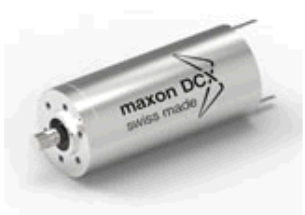
\includegraphics[width=0.3\textwidth]{Figures/Hardware/Partes/DCX32L.png}
\captionof{figure}{Motor DCX32L}
\label{fig:Hardware:Partes:Motor:DCX32L}
\end{center}

%Principio de la tabla GPX32 G1 35:1
%Sensor - ENX16 EASY 1024IMP
\begin{table}[H]
\begin{center}
\begin{tabular}{|l|l|}

\hline
\multicolumn{2}{|c|}{GPX32 G1 35:1}\\ \hline
\multicolumn{2}{|c|}{Funciones}\\ \hline
Gearhead type & \multicolumn{1}{|c|}{Versión estándar}\\ \hline
Redeucción & \multicolumn{1}{|c|}{35:1}\\ \hline
Número de etapas & \multicolumn{1}{|c|}{2}\\ \hline
Conmutación & \multicolumn{1}{|c|}{Graphote brushes}\\ \hline
Fuente de voltaje & \multicolumn{1}{|c|}{Voltaje nominal 12[V]}\\ \hline
Motor bearings & \multicolumn{1}{|c|}{preloaded ball bearing}\\ \hline
Conteos por vuelta & \multicolumn{1}{|c|}{1024}\\ \hline
Hysteresis & \multicolumn{1}{|c|}{0.17m}\\ \hline
\multicolumn{2}{|c|}{Forma y ajuste}\\ \hline
Gear shaft & \multicolumn{1}{|c|}{With flat}\\ \hline
Shaft bore & \multicolumn{1}{|c|}{Without transverse bore}\\ \hline
Shaft length L1 & \multicolumn{1}{|c|}{21[mm]}\\ \hline
Length of flat L2 & \multicolumn{1}{|c|}{12[mm]}\\ \hline
Height of flat D2 & \multicolumn{1}{|c|}{7[mm]}\\ \hline
Gear flange & \multicolumn{1}{|c|}{Standard flange}\\ \hline
Amount of threads & \multicolumn{1}{|c|}{4}\\ \hline
Thread diameter & \multicolumn{1}{|c|}{M3}\\ \hline
Pitch circle diameter TK & \multicolumn{1}{|c|}{26[mm]}\\ \hline
Conexión eléctrica, motor & \multicolumn{1}{|c|}{cable}\\ \hline
Tipo de conector, motor & \multicolumn{1}{|c|}{Sin conector}\\ \hline
Longitud del cable L1 para el motor & \multicolumn{1}{|c|}{200[mm]}\\ \hline
Tipo de cable & \multicolumn{1}{|c|}{AWG18}\\ \hline
Conexión electrica, enconder & \multicolumn{1}{|c|}{Estándar}\\ \hline
Longitud del cable L1 para el encoder & \multicolumn{1}{|c|}{200[mm]}\\ \hline
Tipo de cable para el enconder & \multicolumn{1}{|c|}{TPE ribbon cable}\\ \hline
Tipo de conector, encoder & \multicolumn{1}{|c|}{10-pol 2.54[mm] pin}\\ \hline
Orientación de la conexión (motor) & \multicolumn{1}{|c|}{0 grados}\\ \hline
Orientación de la conexión (enconder) & \multicolumn{1}{|c|}{0 grados}\\ \hline
\multicolumn{2}{|c|}{Your entries}\\ \hline
Voltaje disponible & \multicolumn{1}{|c|}{12[V]}\\ \hline
Velocidad & \multicolumn{1}{|c|}{180[rpm]}\\ \hline
Torque & \multicolumn{1}{|c|}{2000[mNm]}\\ \hline
\multicolumn{2}{|c|}{Valores de el dispositivo con voltaje}\\ \hline
Máx. speed at given load & \multicolumn{1}{|c|}{190[rpm]}\\ \hline
Máximo torque continuo & \multicolumn{1}{|c|}{2440.62[mNm]}\\ \hline
Máxima corriente continua & \multicolumn{1}{|c|}{6[A]}\\ \hline



\end{tabular}
\caption{GPX32 G1 35:1}
\label{GPX32 G1 }
\end{center}
\end{table}
%Fin de la tabla

%Principio de la tabla GPX32 LN 16:1
%Sensor - ENX16 EASY 1024IMP
\begin{table}[H]
\begin{center}
\begin{tabular}{|l|l|}

\hline
\multicolumn{2}{|c|}{GPX32 G1 16:1}\\ \hline
\multicolumn{2}{|c|}{Funciones}\\ \hline
Gearhead type & \multicolumn{1}{|c|}{Nivel de ruido reducido}\\ \hline
Redeucción & \multicolumn{1}{|c|}{16:1}\\ \hline
Número de etapas & \multicolumn{1}{|c|}{2}\\ \hline
Conmutación & \multicolumn{1}{|c|}{Graphote brushes}\\ \hline
Fuente de voltaje & \multicolumn{1}{|c|}{Voltaje nominal 12[V]}\\ \hline
Motor bearings & \multicolumn{1}{|c|}{preloaded ball bearing}\\ \hline
Conteos por vuelta & \multicolumn{1}{|c|}{1024}\\ \hline
Hysteresis & \multicolumn{1}{|c|}{0.17m}\\ \hline
\multicolumn{2}{|c|}{Forma y ajuste}\\ \hline
Gear shaft & \multicolumn{1}{|c|}{With flat}\\ \hline
Shaft bore & \multicolumn{1}{|c|}{Without transverse bore}\\ \hline
Shaft length L1 & \multicolumn{1}{|c|}{21[mm]}\\ \hline
Length of flat L2 & \multicolumn{1}{|c|}{12[mm]}\\ \hline
Height of flat D2 & \multicolumn{1}{|c|}{7[mm]}\\ \hline
Gear flange & \multicolumn{1}{|c|}{Standard flange}\\ \hline
Amount of threads & \multicolumn{1}{|c|}{4}\\ \hline
Thread diameter & \multicolumn{1}{|c|}{M3}\\ \hline
Pitch circle diameter TK & \multicolumn{1}{|c|}{26[mm]}\\ \hline
Conexión eléctrica, motor & \multicolumn{1}{|c|}{Terminal (bent radially)}\\ \hline
Conexión electrica, enconder & \multicolumn{1}{|c|}{Estándar}\\ \hline
Longitud del cable L1 para el encoder & \multicolumn{1}{|c|}{200[mm]}\\ \hline
Tipo de cable para el enconder & \multicolumn{1}{|c|}{TPE ribbon cable}\\ \hline
Tipo de conector, encoder & \multicolumn{1}{|c|}{10-pol 2.54[mm] pin}\\ \hline
Orientación de la conexión (motor) & \multicolumn{1}{|c|}{0 grados}\\ \hline
Orientación de la conexión (enconder) & \multicolumn{1}{|c|}{0 grados}\\ \hline
\multicolumn{2}{|c|}{Your entries}\\ \hline
Voltaje disponible & \multicolumn{1}{|c|}{12[V]}\\ \hline
Velocidad & \multicolumn{1}{|c|}{400[rpm]}\\ \hline
Torque & \multicolumn{1}{|c|}{900[mNm]}\\ \hline
\multicolumn{2}{|c|}{Valores de el dispositivo con voltaje}\\ \hline
Máx. speed at given load & \multicolumn{1}{|c|}{417[rpm]}\\ \hline
Máximo torque continuo & \multicolumn{1}{|c|}{1115.71[mNm]}\\ \hline
Máxima corriente continua & \multicolumn{1}{|c|}{6[A]}\\ \hline

\end{tabular}
\caption{Motor DCX32L}
\label{Motor DCX32L}
\end{center}
\end{table}
%Fin de la tabla

%Principio de la tabla
\begin{table}[H]
\begin{center}
\begin{tabular}{|l|l|}%Define el número de columnas

\hline
\multicolumn{2}{|c|}{Motor - DCX32L GB KL 12V} \\ \hline %Une un renglon completo 
\multicolumn{2}{|c|}{Valores en voltaje nominal} \\ \hline %Une un renglon completo 
Voltaje nominal &  \multicolumn{1}{|c|}{12[V]}\\ \hline
Velocidad sin carga  & \multicolumn{1}{|c|}{7120[rpm]}\\ \hline
Corriente sin carga & \multicolumn{1}{|c|}{274[mA]}\\ \hline
Velocidad nominal & \multicolumn{1}{|c|}{6560[rpm]}\\ \hline
Torque nominal (máx. torque continuo) & \multicolumn{1}{|c|}{89.4[mNm]}\\ \hline
Corriente nominal & \multicolumn{1}{|c|}{6[A]}\\ \hline
Stall Torque & \multicolumn{1}{|c|}{1730[mNm]}\\ \hline
Stall Corriente & \multicolumn{1}{|c|}{111[A]}\\ \hline
Eficiencia máxima & \multicolumn{1}{|c|}{85.5\%}\\ \hline
\multicolumn{2}{|c|}{Caracteristicas} \\ \hline %Une un renglon completo 
Máxima salida de potencia & \multicolumn{1}{|c|}{90.2[W]}\\ \hline
Resistencia de terminal & \multicolumn{1}{|c|}{0.108[Ohm]}\\ \hline
Inductancía de terminal & \multicolumn{1}{|c|}{0.03362[mH]}\\ \hline
Torque constante & \multicolumn{1}{|c|}{15.6[mNm/A]}\\ \hline
Velocidad constante & \multicolumn{1}{|c|}{612[rpm/V]}\\ \hline
Gradiente de velocidad/torque & \multicolumn{1}{|c|}{4.24[rpm/mNm]}\\ \hline
Mechanical time constant & \multicolumn{1}{|c|}{3.44[ms]}\\ \hline
Inercia del rotor & \multicolumn{1}{|c|}{77.6[gcm\^2]}\\ \hline
\multicolumn{2}{|c|}{Datos termicos} \\ \hline %Une un renglon completo 
Resistencia termica housing-ambient & \multicolumn{1}{|c|}{7.28[K/W]}\\ \hline
Resistencia termica winding-housing & \multicolumn{1}{|c|}{2.3[K/W]}\\ \hline
Thermal time constant 0f the winding & \multicolumn{1}{|c|}{45[s]}\\ \hline
Constante de tiempo termica del motor & \multicolumn{1}{|c|}{837[s]}\\ \hline
Temperatura ambiente & \multicolumn{1}{|c|}{-40 a 100[Grados C]}\\ \hline
Max. winding temperatura & \multicolumn{1}{|c|}{155[grados C]}\\ \hline
\multicolumn{2}{|c|}{Datos mecanicos} \\ \hline %Une un renglon completo 
Velocidad máxima permisible & \multicolumn{1}{|c|}{11300[rpm]}\\ \hline
Min. axial play & \multicolumn{1}{|c|}{0[mm]}\\ \hline
Máx. axial play & \multicolumn{1}{|c|}{0.1[mm]}\\ \hline
Radial backlash & \multicolumn{1}{|c|}{0.02[mm]}\\ \hline
Max. axial load (dynamic) & \multicolumn{1}{|c|}{7[N]}\\ \hline
Max. force for press fits & \multicolumn{1}{|c|}{22.6[N]}\\ \hline
Max. radial load & \multicolumn{1}{|c|}{65.3[N]}\\ \hline
\multicolumn{2}{|c|}{Especificaciones} \\ \hline %Une un renglon completo
Número de pares de polos & \multicolumn{1}{|c|}{1}\\ \hline
Número de segmentos del conmutador & \multicolumn{1}{|c|}{11}\\ \hline
Peso & \multicolumn{1}{|c|}{0[mm]}\\ \hline
Nivel de ruido tipico & \multicolumn{1}{|c|}{47dbA}\\ \hline



\end{tabular}
\caption{Motor DCX32L}
\label{Motor DCX32L}
\end{center}
\end{table}
%Fin de la tabla


\subsection{USB2Dynamixel adapter}

%Figura del Dynamixel
\begin{center}
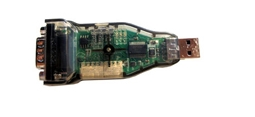
\includegraphics[width=0.6\textwidth]{Figures/Hardware/Partes/Dynamixel.png}
\captionof{figure}{Adaptador USBDynamixel}
\label{fig:Hardware:Partes:Dynamixel}
\end{center}

Para controlar una red de Robotics Dynamixels desde el puerto USB de la computadora\\
El adaptador USB2Dynamixel tiene tres opciones de salida:\\
\\
-Nivel TTL RS232: conector de 3 pines, usado con un Dynamixel serie AX y MX-T\\
 \begin{itemize}
\item{AX-12A}
\item{AX-18A}
\item{AX-12W}
\item{MX-28T}
\item{MX-64T}
\item{MX-106T}
\\
\end{itemize}
-S485: conector de 4 pines, usado con RX, EX y MX-R de la serie Dynamixel\\

\begin{itemize}
\item{RX-24F}
\item{RX-28}
\item{RX-64}
\item{RX-28R}
\item{MX-64R}
\item{MX-106R}
\item{EX-106}
\end{itemize}

\subsection{Roboclaw 2x30A}

%Figura
\begin{center}
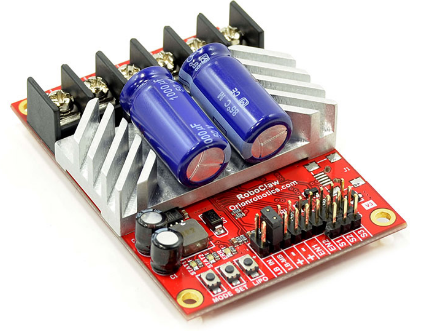
\includegraphics[width=0.4\textwidth]{Figures/Hardware/Partes/Roboclaw_2x30A.png}
\captionof{figure}{Roboclaw 2x30A}
\label{fig:Hardware:Partes:Roboclaw:2x30A}
\end{center}


%Principio de la tabla
\begin{table}[H]
\begin{center}
\begin{tabular}{|l|l|}%Define el número de columnas


\hline
\multicolumn{2}{|c|}{Roboclaw 2x30A} \\ \hline %Une un renglon completo 
Canales para motor & \multicolumn{1}{|c|}{2}\\ \hline
Voltaje de operacion & \multicolumn{1}{|c|}{6[V] a 34[V]}\\ \hline
corriente continua de salida & \multicolumn{1}{|c|}{20[A]}\\ \hline
pico de corriente de salida & \multicolumn{1}{|c|}{60[A]}\\ \hline
5V BEC(1) corriente máxima & \multicolumn{1}{|c|}{3[A]}\\ \hline
Ancho & \multicolumn{1}{|c|}{5.2[cm]}\\ \hline
Largo & \multicolumn{1}{|c|}{7.4[cm]}\\ \hline
Peso & \multicolumn{1}{|c|}{63[g]}\\ \hline

\end{tabular}
\caption{Roboclaw 2x30A}
\label{Datos del Roboclaw}
\end{center}
\end{table}
%Fin de la tabla

\subsection{Roboclaw 2x15A}

%Figura
\begin{center}
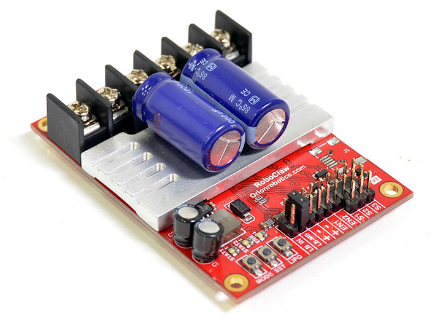
\includegraphics[width=0.5\textwidth]{Figures/Hardware/Partes/Roboclaw_2x15A.png}
\captionof{figure}{Roboclaw 2x15A}
\label{fig:Hardware:Partes:Roboclaw:2x15A}
\end{center}

%Principio de la tabla
\begin{table}[H]
\begin{center}
\begin{tabular}{|l|l|}%Define el número de columnas


\hline
\multicolumn{2}{|c|}{Roboclaw 2x15A} \\ \hline %Une un renglon completo 
Canales para motor & \multicolumn{1}{|c|}{2}\\ \hline
Voltaje de operacion & \multicolumn{1}{|c|}{6[V] a 34[V]}\\ \hline
corriente continua de salida & \multicolumn{1}{|c|}{15[A]}\\ \hline
pico de corriente de salida & \multicolumn{1}{|c|}{30[A]}\\ \hline
5V BEC(1) corriente máxima & \multicolumn{1}{|c|}{3[A]}\\ \hline
Ancho & \multicolumn{1}{|c|}{5.2[cm]}\\ \hline
Largo & \multicolumn{1}{|c|}{7.4[cm]}\\ \hline
Peso & \multicolumn{1}{|c|}{54[g]}\\ \hline

\end{tabular}
\caption{Roboclaw 2x15A}
\label{Datos del Roboclaw}
\end{center}
\end{table}
%Fin de la tabla

%Empiesan los consejos y conexiones 

\vfill

\section{Vision, navegación y sonido}
\subsection{Kinect}

%Figura
\begin{center}
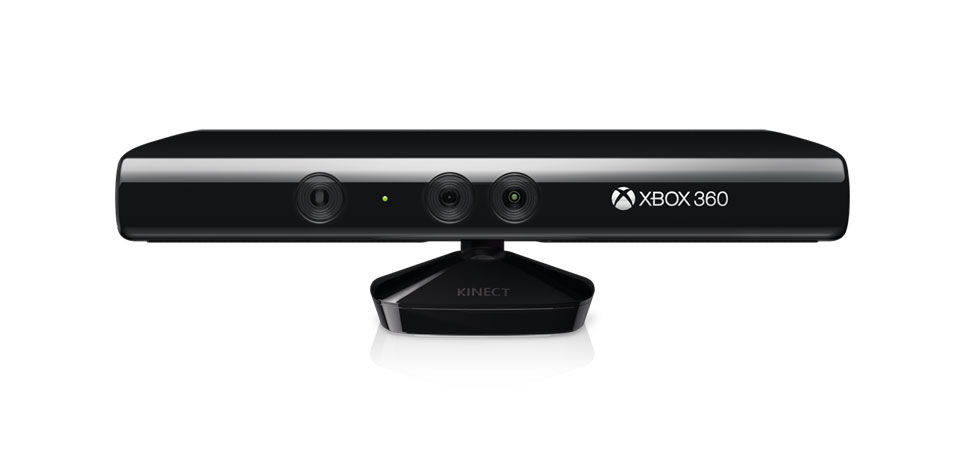
\includegraphics[width=0.7\textwidth]{Figures/Hardware/Partes/Kinect.png}
\captionof{figure}{Kinect}
\label{fig:Hardware:Partes:Kinect}
\end{center}

%Principio de la tabla
\begin{table}[H]
\begin{center}
\begin{tabular}{|l|l|}%Define el número de columnas


\hline
\multicolumn{2}{|c|}{Kinect} \\ \hline %Une un renglon completo 
Caracteristicas & \multicolumn{1}{|c|}{Sensores}\\ \hline
Campo de visión & \multicolumn{1}{|c|}{57.5grados horizontal por 43.5grados vertical}\\ \hline
Profundidad resoluble& \multicolumn{1}{|c|}{0.8[m]->4.0[m]}\\ \hline
\multirow{3}{1cm}{Flujo de color} & \multicolumn{1}{|c|}{640x480x24 bpp 4:3 RGB} \\  & \multicolumn{1}{|c|}{@ 30fps 640x480x16bpp} \\  & \multicolumn{1}{|c|}{4:3 YUV @ 15fps} \\  \hline
Infrarrojo & \multicolumn{1}{|c|}{Sin flujo IR}\\ \hline
Registro & \multicolumn{1}{|c|}{Color <-> ruta}\\ \hline
Ruta de datos & \multicolumn{1}{|c|}{USB 2.0}\\ \hline
Latencia & \multicolumn{1}{|c|}{~90 ms con procesos}\\ \hline
Motor de inclinación & \multicolumn{1}{|c|}{Sólo vertical}\\ \hline

\end{tabular}
\caption{Kinect}
\label{Datos del Kinect}
\end{center}
\end{table}
%Fin de la tabla

\vfill

\subsection{Hokuyo UHG-08LX}

%Figura
\begin{center}
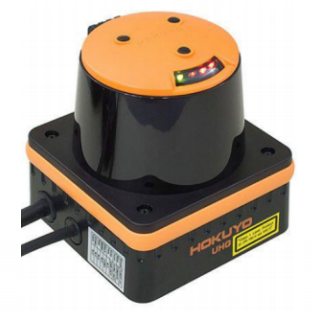
\includegraphics[width=0.35\textwidth]{Figures/Hardware/Partes/Hokuyo.png}
\captionof{figure}{Hokuyo UHG-08LX}
\label{fig:Hardware:Partes:Hokuyo:UHG-08LX}
\end{center}

%Principio de la tabla
\begin{table}[H]
\begin{tabular}{|l|l|}%Define el número de columnas


\hline
\multicolumn{2}{|c|}{Hokuyo UHG-08LX Scanning Laser} \\ \hline %Une un renglon completo 
Alimentación &  \multicolumn{1}{|c|}{12[V]}\\ \hline
Rango de detección & \multicolumn{1}{|c|}{De 20 a 8000[mm]}\\ \hline
Exactitud & \multicolumn{1}{|c|}{De 100 a 1000[mm]}\\ \hline
Resolución angular & \multicolumn{1}{|c|}{0.36grados(360grados/1,024 pasos)}\\ \hline

Fuente de luz & \multicolumn{1}{|c|}{Diodo laser semiconductor }\\ \hline
Tiempo de escaneo & \multicolumn{1}{|c|}{67[msec/scan]}\\ \hline
Nivel de sonido & \multicolumn{1}{|c|}{menos de 25dB}\\ \hline
Interface & \multicolumn{1}{|c|}{USB2.0 (velocidad completa)}\\ \hline
Salida sincrona & \multicolumn{1}{|c|}{NPN colector abierto}\\ \hline
Comando del sistema & \multicolumn{1}{|c|}{Comanda diseñado exclusivamente SCIP ver. 2.0}\\ \hline
Conexión & \multicolumn{1}{|c|}{Salida de voltaje y sincronía: 2}\\ \hline
Iluminación ambiente & \multicolumn{1}{|c|}{Lampara de alogeno/mercurio: 10,000lx o menos, fluorescente: 6,000lx(máx)}\\ \hline
Ambiente (temperatura/humedad) & \multicolumn{1}{|c|}{-10 a 50 [grados C], menos del 85\% RH}\\ \hline
Resistencia a la vibración & \multicolumn{1}{|c|}{Amplitud doble 1.5[mm], de 10 a 55[Hz], 2 veces en cada dirección X, Y y Z}\\ \hline
Resistencia al impacto & \multicolumn{1}{|c|}{196[m/s], 10 veces en las direcciones X, Y y Z}\\ \hline
Peso & \multicolumn{1}{|c|}{Aprox. 500[g](con el cable conectado)}\\ \hline

\end{tabular}
\caption{Hakuyo UHG-08LX}
\label{Datos del Hokuyo}
\end{table}
%Fin de la tabla

\subsection{Microfono RODE}

%Figura
\begin{center}
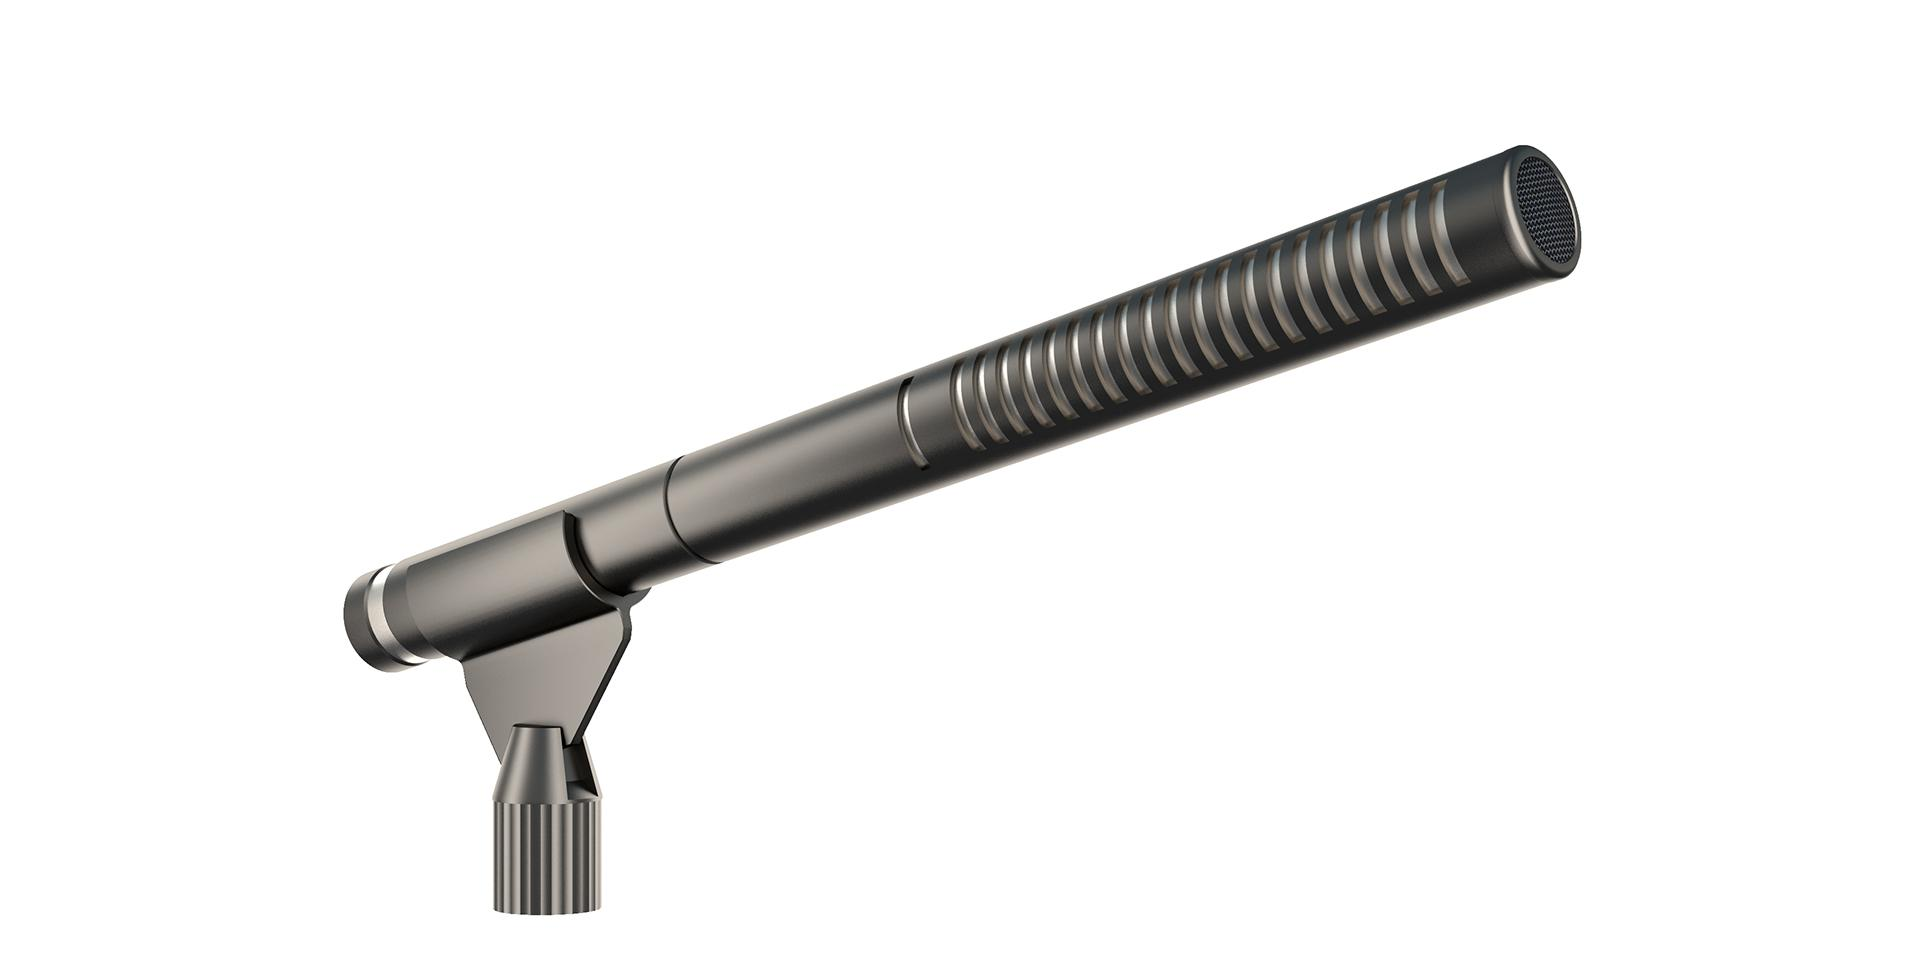
\includegraphics[width=0.6\textwidth]{Figures/Hardware/Partes/Rode.jpg}
\captionof{figure}{Microfono Rode NTG-2}
\label{fig:Hardware:Partes:Microfono:Rode}
\end{center}

%Principio de la tabla

\begin{minipage}{1\textwidth}
\begin{flushleft} %\large
\begin{table}[H]

\begin{tabular}{|l|l|}%Define el número de columnas

\hline
\multicolumn{2}{|c|}{Microfono Rode NTG-2} \\ \hline %Une un renglon completo 
Principio acustico &  \multicolumn{1}{|c|}{Line Gradient}\\ \hline
Electronica & \multicolumn{1}{|c|}{Conversor de impedancia JFET con un transformador de salida balanceado}\\ \hline
Capsula & \multicolumn{1}{|c|}{0.50"}\\ \hline
Tipo de dirección & \multicolumn{1}{|c|}{End}\\ \hline
Rango de frecuencia & \multicolumn{1}{|c|}{20Hz-20kHz}\\ \hline
Impedancia de salida & \multicolumn{1}{|c|}{250[ohms]}\\ \hline
Nivel de sonido & \multicolumn{1}{|c|}{131dB SPL(@ 1kHz, 1\% THD en carga de 1kohm)}\\ \hline
Máximo nivel de salida & \multicolumn{1}{|c|}{6.9[mV]}\\ \hline
Sensibilidad & \multicolumn{1}{|c|}{-36.0dB re 1[Volt/pascal] (15[mV] @ 94dB SPL)+/- 2dB}\\ \hline
Nivel de ruido equivalente & \multicolumn{1}{|c|}{18dB-A}\\ \hline
Opciones de alimentación & \multicolumn{1}{|c|}{Pilas AA o P48}\\ \hline
Peso & \multicolumn{1}{|c|}{161[gm]}\\ \hline
Dimensiones & \multicolumn{1}{|c|}{280[mmH]x22[mmW]x22[mmD]}\\ \hline
Salida & \multicolumn{1}{|c|}{XLR}\\ \hline


\end{tabular}
\caption{Microfono Rode}
\label{Microfono Rode}

\end{table}

\end{flushleft}
\end{minipage}
%Fin de la tabla
\vfill

\section{Alimentación de Justina}

\subsection{Alimentación bateria Li-po}

Para el robot Justina se utilizan 3 baterías conectadas en paralelo

%Figura
\begin{center}
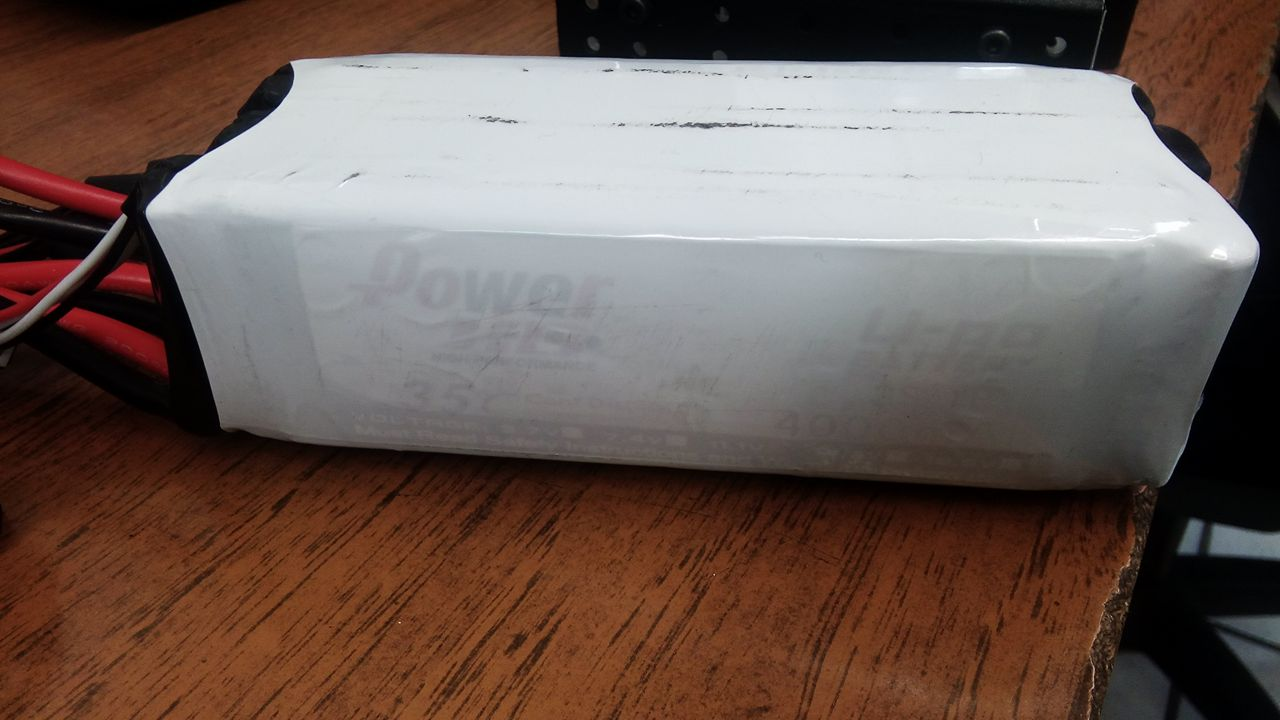
\includegraphics[width=0.5\textwidth]{Figures/Hardware/Partes/Li-po_Battery.jpg}
\captionof{figure}{Bateria Li-po}
\label{fig:Hardware:Partes:Battery}
\end{center}

%Principio de la tabla
\begin{table}[H]
\begin{center}
\begin{tabular}{|l|l|}%Define el número de columnas

\hline
\multicolumn{2}{|c|}{Batería Li-po 4000mAh a 11.1[V]} \\ \hline %Une un renglon completo 
Voltaje &  \multicolumn{1}{|c|}{11.1[V] en 3 celdas}\\ \hline
Corriente de descarga por hora  & \multicolumn{1}{|c|}{4000[mAh]}\\ \hline
Tasa de descarga & \multicolumn{1}{|c|}{35C}\\ \hline
Plug de carga & \multicolumn{1}{|c|}{JST-XH}\\ \hline
Plug de descarga & \multicolumn{1}{|c|}{"T"}\\ \hline
Medidas & \multicolumn{1}{|c|}{25x46x144[mm]}\\ \hline
Peso & \multicolumn{1}{|c|}{335[gr]}\\ \hline

\end{tabular}
\caption{Bateria Li-po}
\label{Battery}
\end{center}
\end{table}
%Fin de la tabla

%

\subsection{ATX configuración}
%Figura
\begin{center}
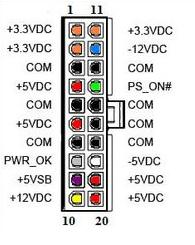
\includegraphics[width=0.4\textwidth]{Figures/Hardware/Partes/ATX.JPG}
\captionof{figure}{Pines ATX}
\label{fig:Hardware:Partes:Microfono:ATX}
\end{center}

\section{HUBs}

\subsection{Cisco-Linksys USB2HUB4 USB 4-Port Hub}

%Figura
\begin{center}
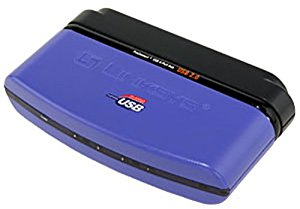
\includegraphics[width=0.5\textwidth]{Figures/Hardware/Partes/Cisco-Linksys.png}
\captionof{figure}{Cisco-Linksys USB2HUB4 USB 4-Port Hub}
\label{fig:Hardware:Partes:Cisco}
\end{center}

%Principio de la tabla
\begin{table}[H]
\begin{center}
\begin{tabular}{|l|l|}%Define el número de columnas


\hline
\multicolumn{2}{|c|}{USB2HUB4} \\ \hline %Une un renglon completo 
\multirow{3}{1cm}{Estándar} & \multicolumn{1}{|c|}{OHCI}\\ & \multicolumn{1}{|c|}{UHIC}\\ & \multicolumn{1}{|c|}{USB 1.1}\\ & \multicolumn{1}{|c|}{USB 2.0}\\ \hline
Puertos & \multicolumn{1}{|c|}{USB type B Root port}\\ &\multicolumn{1}{|c|}{4 USB type A device ports}\\ \hline
Número máximo de dispositivos & \multicolumn{1}{|c|}{127}\\ \hline
Cable & \multicolumn{1}{|c|}{Shielded USB 2.0}\\ \hline
\multicolumn{2}{|c|}{Environmental}\\ \hline
Dimensiones & \multicolumn{1}{|c|}{4.52"x0.75"x2.675"}\\ \hline
Masa & \multicolumn{1}{|c|}{70[g]}\\ \hline
Alimentación & \multicolumn{1}{|c|}{5[V] DC a 2.4[A]}\\ \hline
Temperatura de operación & \multicolumn{1}{|c|}{0 a 70 grados}\\ \hline
Temperatura en almacenamiento & \multicolumn{1}{|c|}{-20 a 176 grados}\\ \hline
Humedad de operación & \multicolumn{1}{|c|}{0 a 95\% sin condensación}\\ \hline
Humedad en almacenamiento & \multicolumn{1}{|c|}{0 a 95\% sin condensación}\\ \hline

\end{tabular}
\caption{USB2HUB4}
\label{Datos del USB2HUB4}
\end{center}
\end{table}
%Fin de la tabla

\subsection{HUB Startech ST4300PBU3}


\begin{center}
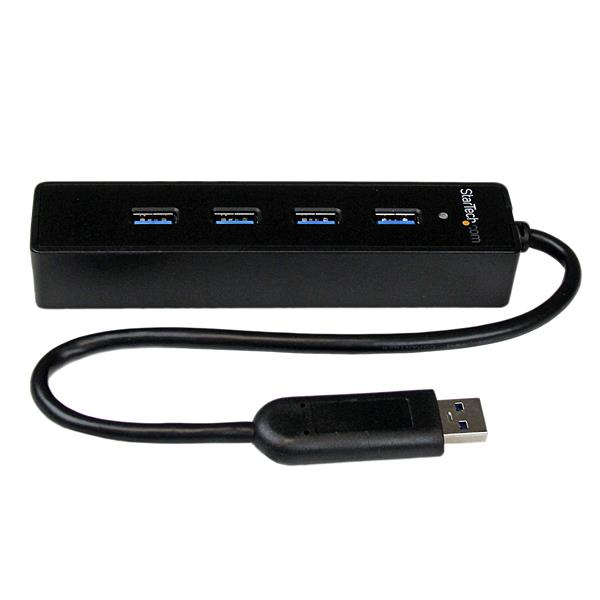
\includegraphics[width=0.5\textwidth]{Figures/Hardware/Partes/ST4300PBU3.jpg}
\captionof{figure}{HUB Startech ST4300PBU3}
\label{fig:Hardware:Partes:HUBST}
\end{center}

%Principio de la tabla
\begin{table}[H]
\begin{center}
\begin{tabular}{|l|l|}%Define el número de columnas


\hline
\multicolumn{2}{|c|}{USB2HUBST4300PBU3} \\ \hline %Une un renglon completo 
\multicolumn{2}{|c|}{Hardware} \\ \hline %Une un renglon completo
Tipo de Bus & \multicolumn{1}{|c|}{USB 3.0}\\ \hline
Chipset ID & \multicolumn{1}{|c|}{VLI-VL812}\\ \hline
Interface & \multicolumn{1}{|c|}{USB 3.0}\\ \hline
Puertos & \multicolumn{1}{|c|}{4}\\ \hline
\multicolumn{2}{|c|}{Rendimiento}\\ \hline
Rango máximo de transferencia de datos & \multicolumn{1}{|c|}{5Gbps}\\ \hline
Tipo y rango & \multicolumn{1}{|c|}{USB 3.0-5Gbit/s}\\ \hline
\multicolumn{2}{|c|}{Conectores}\\ \hline
Puertos externos & \multicolumn{1}{|c|}{1-USB tipo A (9 pines) USB 3.0 macho}\\ & \multicolumn{1}{|c|}{4-USB tipo A (9 pines) USB 3.0 hembra}\\ \hline
\multicolumn{2}{|c|}{Software}\\ \hline
Compatibilidad con SO & \multicolumn{1}{|c|}{SO independiente; Sin software o drivers adicionales requeridos}\\ \hline
\multicolumn{2}{|c|}{Notas especiales/Requerimientos}\\ \hline
Requerimientos de sistema y cables & \multicolumn{1}{|c|}{Puerto USB disponible}\\ \hline
\multicolumn{2}{|c|}{Indicadores}\\ \hline
LED indicador & \multicolumn{1}{|c|}{1 - power}\\ \hline
\multicolumn{2}{|c|}{Power}\\ \hline
Fuente de poder & \multicolumn{1}{|c|}{USB-Powered}\\ \hline
\multicolumn{2}{|c|}{Entorno}\\ \hline
Humedad & \multicolumn{1}{|c|}{20~80\% RH}\\ \hline
Temperatura de operación & \multicolumn{1}{|c|}{-5 grados C a 45 gradosC}\\ \hline
Temperatura en alamacenamiento & \multicolumn{1}{|c|}{-10 grados C a 75 grados C}\\ \hline
 
\end{tabular}
\caption{USB2HUB4}
\label{Datos del USB2HUB4}
\end{center}
\end{table}
%Fin de la tabla

 
\end{document}
